\documentclass[a4paper,12pt]{article} 

% First, we usually want to set the margins of our document. For this we use the package geometry.
\usepackage[top = 2.5cm, bottom = 2.5cm, left = 2.5cm, right = 2.5cm]{geometry} 
\usepackage[T1]{fontenc}
\usepackage[utf8]{inputenc}

% The following two packages - multirow and booktabs - are needed to create nice looking tables.
\usepackage{multirow} % Multirow is for tables with multiple rows within one cell.
\usepackage{booktabs} % For even nicer tables.

% As we usually want to include some plots (.pdf files) we need a package for that.
\usepackage{graphicx} 

% The default setting of LaTeX is to indent new paragraphs. This is useful for articles. But not really nice for homework problem sets. The following command sets the indent to 0.
%\usepackage{setspace}
%\setlength{\parindent}{0in}
\usepackage{indentfirst}

% Package to place figures where you want them.
\usepackage{float}

% The fancyhdr package let's us create nice headers.
\usepackage{fancyhdr}

\usepackage{amsmath,amsthm}

% To make our document nice we want a header and number the pages in the footer.

\pagestyle{fancy} % With this command we can customize the header style.

\fancyhf{} % This makes sure we do not have other information in our header or footer.

\lhead{\footnotesize Data Structure and Algorithm Analysis(H): Work Sheet 5}% \lhead puts text in the top left corner. \footnotesize sets our font to a smaller size.

%\rhead works just like \lhead (you can also use \chead)
\rhead{\footnotesize Mengxuan Wu} %<---- Fill in your lastnames.

% Similar commands work for the footer (\lfoot, \cfoot and \rfoot).
% We want to put our page number in the center.
\cfoot{\footnotesize \thepage} 

\begin{document}

\thispagestyle{empty} % This command disables the header on the first page. 

\begin{tabular}{p{15.5cm}}
{\large \bf Data Structure and Algorithm Analysis(H)} \\
Southern University of Science and Technology \\ Mengxuan Wu \\ 12212006 \\
\hline
\\
\end{tabular}

\vspace*{0.3cm} %add some vertical space in between the line and our title.

\begin{center}
	{\Large \bf Work Sheet 5}
	\vspace{2mm}

	{\bf Mengxuan Wu}
		
\end{center}  

\vspace{0.4cm}

\section*{Question 5.1}

\begin{figure}[H]
	\centering
	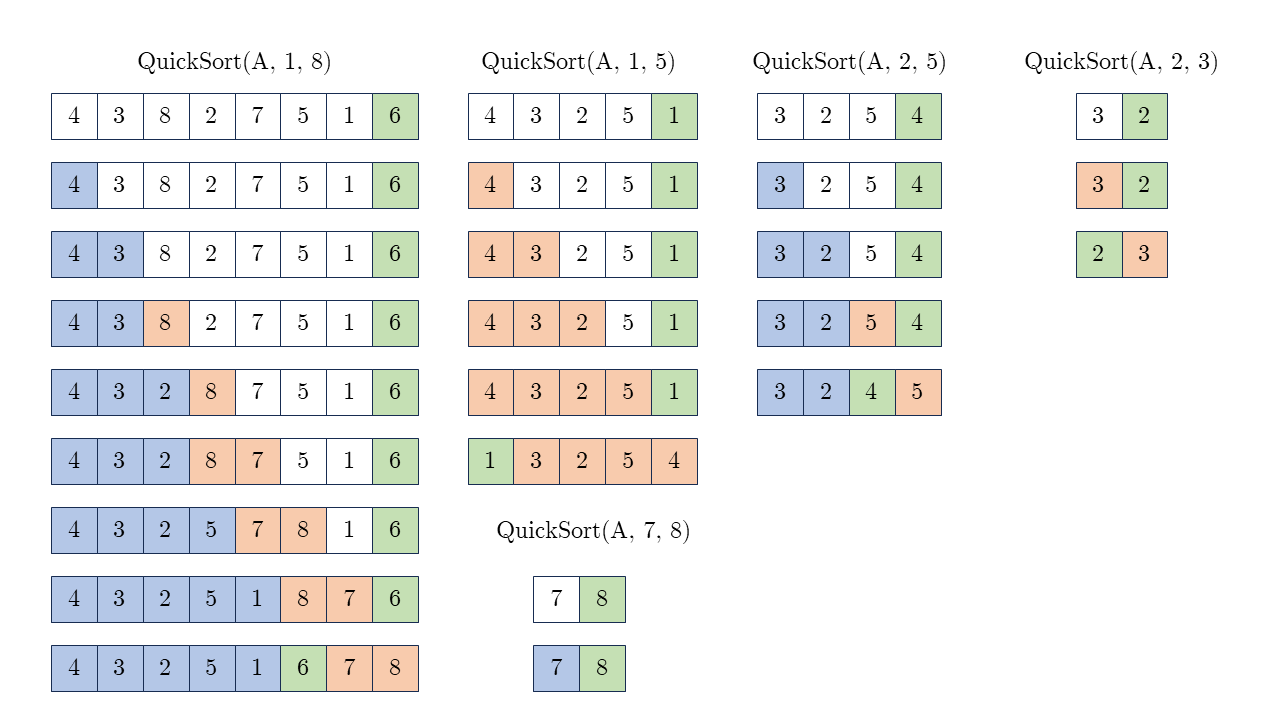
\includegraphics[width=0.9\textwidth]{Figure 1/幻灯片1.PNG}
\end{figure}

\textit{Note: I omit all subarrays of size 0 or 1 in the figure.}
\section*{Question 5.2}

\begin{center}
	\begin{tabular}{ll}
		\toprule
		\multicolumn{2}{l}{\textsc{QuickSort}$(A,p,r)$}\\
		\midrule
		1. & \textbf{if} $p<r$ \textbf{then}\\
		2. & \qquad $q$ = \textsc{Partition}$(A,p,r)$\\
		3. & \qquad \textsc{QuickSort}$(A,p,q-1)$\\
		4. & \qquad \textsc{QuickSort}$(A,q+1,r)$\\
		\bottomrule
	\end{tabular}
\end{center}

To proof the correctness of the algorithm, we need to proof by induction.

\textbf{Base case:} Let $n = r - p + 1$ be the size of input. 
If $n = 1$, then the array is already sorted.
So the base case holds.

\textbf{Inductive case:} Assume that the algorithm works for all input of size $n < c$.
Now we need to proof that the algorithm works for input of size $n = c$.

Since \textsc{Partition} is correct, we know that the array is partitioned into two parts, $A[p\dots q-1]$ and $A[q+1\dots r]$, where $A[p\dots q-1] \leq A[q] \leq A[q+1\dots r]$.
By the inductive hypothesis, we know that \textsc{QuickSort}$(A,p,q-1)$ and \textsc{QuickSort}$(A,q+1,r)$ will sort the two parts, since the size of the two parts are less than $c$.
So the whole array will be sorted.

\section*{Question 5.3}

When the array of distinct elements is sorted in decreasing order, the pivot will always be the smallest element in the array.
Therefore, the partition will always give the pivot the index $p$.
And the two subarray will always be $A[p\dots p - 1]$ (which is an empty array) and $A[p + 1\dots r]$ (which excludes only the pivot).
So the size of the two subarray are $0$ and $n - 1$.

Hence, the recurrence relation is $T(n) = T(0) + T(n - 1) + \Theta(n)$, which is the same as that of array sorted in increasing order.
Therefore, the runtime of \textsc{QuickSort} when the array contains distinct elements in decreasing order is $\Theta(n^2)$.

\section*{Question 5.4}

When all $n$ elements have the same value, the partition will always give the pivot the index $r$.

For such an input, the recurrence relation is $T(n) = T(n - 1) + T(0) + \Theta(n)$, which is the same as that of array sorted in increasing order.
Therefore, the runtime is $\Theta(n^2)$.

\section*{Question 5.5}
\begin{minipage}{0.5\textwidth}
	\begin{center}
		\begin{tabular}{ll}
			\toprule
			\multicolumn{2}{l}{\textsc{Partition'}$(A,p,r)$}\\
			\midrule
			1. & $x = A[r]$\\
			2. & $i = p - 1$\\
			3. & $k = p - 1$\\
			4. & \textbf{for} $j = p$ \textbf{to} $r - 1$ \textbf{do}\\
			5. & \qquad \textbf{if} $A[j] < x$ \textbf{then}\\
			6. & \qquad \qquad $i = i + 1$\\
			7. & \qquad \qquad $k = k + 1$\\
			8. & \qquad \qquad exchange $A[i]$ with $A[j]$\\
			9. & \qquad \qquad \textbf{if} $i \neq k$ \textbf{then}\\
			10. & \qquad \qquad \qquad exchange $A[k]$ with $A[j]$\\
			11. & \qquad \textbf{else if} $A[j] = x$ \textbf{then}\\
			12. & \qquad \qquad $k = k + 1$\\
			13. & \qquad \qquad exchange $A[k]$ with $A[j]$\\
			14. & exchange $A[k + 1]$ with $A[r]$\\
			15. & \textbf{return} $i + 1, k + 1$\\
			\bottomrule
		\end{tabular}
	\end{center}
\end{minipage}
\begin{minipage}{0.5\textwidth}
	\begin{center}
		\begin{tabular}{ll}
			\toprule
			\multicolumn{2}{l}{\textsc{QuickSort'}$(A,p,r)$}\\
			\midrule
			1. & \textbf{if} $p<r$ \textbf{then}\\
			2. & \qquad $q_1, q_2$ = \textsc{Partition'}$(A,p,r)$\\
			3. & \qquad \textsc{QuickSort'}$(A,p,q_1-1)$\\
			4. & \qquad \textsc{QuickSort'}$(A,q_2+1,r)$\\
			\bottomrule
		\end{tabular}
	\end{center}
\end{minipage}

The modified \textsc{Partition'} will run in $\Theta(n)$ time, since it runs through the array once and every operation in or out of the for loop takes constant time.

The runtime of \textsc{QuickSort'} on the input of question 5.4 is $\Theta(n)$, since the partition will be executed once and both of the two subarrays will be of size $0$.
\end{document}